\section{Results I: Digital Twin Fidelity}
\label{sec:results_fidelity}

This section answers the question \emph{``How accurate is the surrogate as
a model of the building?''} It deliberately does \emph{not} answer
``Does it train good RL controllers?'' --- that question is addressed in
Section~\ref{sec:results_control}.

\subsection{Architecture comparison}
\label{ssec:res1_architecture}

Table~\ref{tab:architecture} compares the three surrogate variants used
throughout this paper. The data-driven \texttt{v3} model has no
identifiable physical parameter; the calibrated \texttt{v3.5} model
exposes $\czon$ explicitly through Stage~B; and the canonical
\texttt{hybrid\_l010} backend uses \texttt{v3.5} only as a regulariser
($\lambda_{\mathrm{temp}}=0.10$, $\lambda_{\mathrm{power}}=5\times10^{-5}$)
without admitting it into the policy's forward pass. The same table
also previews the closed-loop transfer numbers that will be developed
in Section~\ref{sec:results_control}: pure \texttt{v3} and
\texttt{hybrid\_l010} both reach sub-degree live RMSE on the peak and
typical heating windows, while pure \texttt{v3.5} exceeds
$\mathbf{4\,^{\circ}\mathrm{C}}$ on both --- the divergence between
predictive accuracy and RL training utility that motivates the rest
of the paper.

\begin{table}[t]
  \centering
  \caption{Architecture comparison of the three surrogate variants. \texttt{v3} is a data-driven feed-forward model on direct-TSup trajectories; \texttt{v35\_calibrated} is the physically informed RC-NeuralODE after Stage A/B/C calibration with explicit zone thermal capacitance $\czon$; \texttt{hybrid\_l010} is the canonical hybrid backend ($\lambda_{\mathrm{temp}}=0.10$, $\lambda_{\mathrm{power}}=5\times10^{-5}$). Block~1 fidelity columns are reproduced from \texttt{reports/block1\_surrogate\_final\_metrics.csv}; live-transfer and divergence columns from \texttt{outputs/block13\_*}.}
  \label{tab:architecture}
  \begin{tabular}{lccccccc}
    \toprule
    & Explicit & Block~1 & Block~1 & Peak & Typical & Peak transfer & Typical transfer\\
    Variant & $\czon$ & 1-step RMSE & 24h RMSE & $\msmetric$ & $\msmetric$ & RMSE\,(\si{\celsius}) & RMSE\,(\si{\celsius})\\
    \midrule
    \texttt{v3} & no & --- & --- & 0.073 & 0.095 & 0.894 & 0.745 \\
    \texttt{v3.5} calibrated & yes & 0.232 & 0.644 & 1.046 & 1.102 & 4.320 & 4.401 \\
    \texttt{hybrid\_l010} & regularizer-only & --- & --- & 0.087 & 0.041 & 0.633 & 0.612 \\
    \bottomrule
  \end{tabular}
\end{table}


\subsection{Replicative validity}
\label{ssec:res1_replicative}

On the one-step replicative metric (Supplementary Table~S11),
calibration reduces the temperature RMSE from
$\SI{0.374}{\celsius}$ to $\SI{0.232}{\celsius}$, a $38\%$
improvement. The companion power head shows the same pattern: the
mean absolute power error falls from $\SI{807.8}{\watt}$ to
$\SI{482.0}{\watt}$, a $40\%$ reduction. Both numbers are reproduced
directly from
\texttt{reports/block1\_surrogate\_final\_metrics.csv} (category
\texttt{inverse\_calibration:best\_temp\_alignment}). The
improvements are consistent with the expectation that explicit
identification of $\czon$ centres the residual distribution
(Section~\ref{ssec:res1_predictive}) and that the Stage~C residual
heads then absorb the remaining non-RC dynamics.

\paragraph{Identification of $\czon$.}
The calibrated zone thermal capacitance is
$\czon = \SI{4.413e5}{\joule\per\kelvin}$, deviating from the synthetic prior
$\czon^{(0)} = \SI{5.3e5}{\joule\per\kelvin}$ by approximately $21\%$. The
estimate is stable across training; the final value is frozen in the
canonical checkpoint and reused unchanged in all downstream experiments.

\subsection{Predictive validity}
\label{ssec:res1_predictive}

Table~\ref{tab:predictive} reports temperature rollout RMSE at
$1\,\mathrm{h}$, $4\,\mathrm{h}$, $8\,\mathrm{h}$, and $24\,\mathrm{h}$
horizons on the held-out prepared corpus. Three observations follow.
First, calibration roughly halves the RMSE at every horizon: from
$\sim\!1.49\,^{\circ}\mathrm{C}$ in the raw model to
$\sim\!0.65\,^{\circ}\mathrm{C}$ in the calibrated model, with no
horizon-dependent crossover. Second, the calibrated model's RMSE is
essentially flat from $1\,\mathrm{h}$ to $24\,\mathrm{h}$
($0.65\to0.64\,^{\circ}\mathrm{C}$), which is the signature of a
correctly identified physical dynamics rather than a model that
accumulates integration error with horizon. Third, the raw model's
RMSE is also flat ($\sim\!1.49\,^{\circ}\mathrm{C}$ at every
horizon), which indicates a systematic bias rather than divergent
dynamics --- the kind of error pattern that improved data alone
would not fix but staged inverse calibration does.

\begin{table}[t]
  \centering
  \caption{Predictive validity of the calibrated physical twin \texttt{v3.5} versus the uncalibrated baseline \texttt{raw\_v35} across rollout horizons. Values are computed on the held-out prepared $15$-minute corpus (8~episodes). Calibration roughly halves the temperature RMSE at every horizon and the RMSE is nearly flat from 1\,h to 24\,h, indicating that the identified $\czon$ produces a stable physical model rather than one that accumulates error with horizon. Source: \texttt{reports/hou\_evins\_predictive\_validity\_table.csv}, originally from \texttt{outputs/surrogate\_v35\_rollout\_prepared\_15min\_*/horizon\_metrics.csv}.}
  \label{tab:predictive}
  \begin{tabular}{llcccc}
    \toprule
    Variant & Metric & 1h & 4h & 8h & 24h \\
    \midrule
    \texttt{raw\_v35} & RMSE\,(\si{\celsius}) & 1.491 & 1.491 & 1.491 & 1.466 \\
     & MAE\,(\si{\celsius}) & 1.236 & 1.236 & 1.236 & 1.221 \\
    \midrule
    \texttt{v35\_calibrated} & RMSE\,(\si{\celsius}) & 0.655 & 0.648 & 0.649 & 0.644 \\
     & MAE\,(\si{\celsius}) & 0.490 & 0.486 & 0.486 & 0.482 \\
    \bottomrule
  \end{tabular}
\end{table}


Figure~\ref{fig:block1} visualizes the two-faced character of the
calibrated physical twin. Panel~(a) shows the multi-horizon predictive
validity advantage: calibration reduces the rollout temperature RMSE by
roughly $56\%$ at every horizon and the curve is nearly flat in the
horizon, which is consistent with a correctly identified physical
dynamics rather than a model that accumulates error. Panel~(b) shows
that the same calibrated model is the \emph{worst}, not the best, when
the held-out predictive metric is replaced by the closed-loop live
\boptest{} transfer metric: the ratio between the two metrics on
\texttt{v3.5\_calibrated} exceeds $6\times$. This gap is the central
empirical motivation for the hybrid construction introduced in
Section~\ref{ssec:method_hybrid}.

\begin{figure}[t]
  \centering
  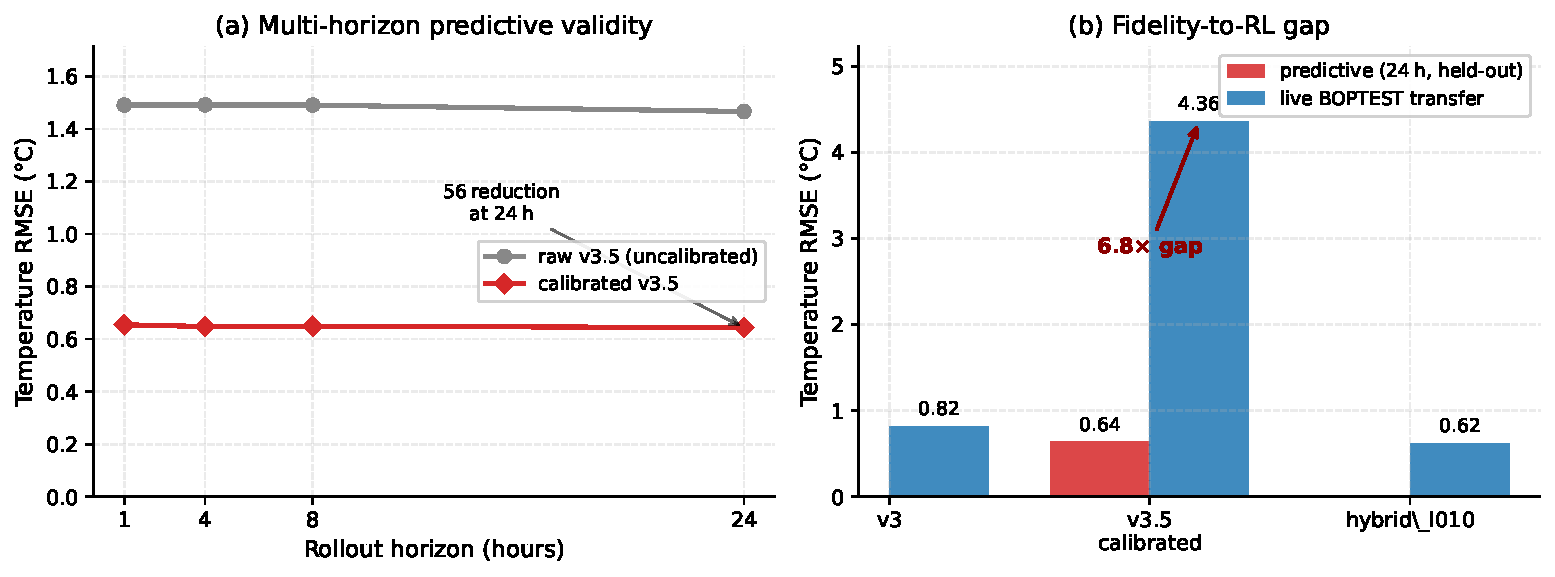
\includegraphics[width=0.95\linewidth]{figures/fig_block1_surrogates.pdf}
  \caption{Block 1 surrogate fidelity. (a) Multi-horizon predictive
  validity on the held-out prepared 15-minute rollout corpus: calibrated
  \texttt{v3.5} achieves a roughly $56\%$ RMSE reduction over its
  uncalibrated baseline at every horizon, and the curve is nearly flat
  from 1\,h to 24\,h. (b) Fidelity-to-RL gap: the same calibrated
  \texttt{v3.5} that wins on predictive validity loses on closed-loop
  \boptest{} transfer, indicating that predictive accuracy alone does
  not deliver a usable RL training environment.}
  \label{fig:block1}
\end{figure}

\subsection{Failure mode: predictive twin is not an RL training environment}
\label{ssec:res1_failure_mode}

The strong predictive validity of \texttt{v3.5} does not transfer to its
usefulness as a closed-loop RL training environment. When a PPO controller
is trained with \texttt{v3.5} as the sole environment and then deployed on
live \boptest, the closed-loop temperature RMSE exceeds \SI{4}{\celsius} on
both heating scenarios ($\SI{4.32}{\celsius}$ on the peak window and
$\SI{4.40}{\celsius}$ on the typical window; see Table~\ref{tab:architecture}
and Supplementary Table~S11 rows \texttt{v35\_calibrated},
\texttt{predictive\_transfer}, \texttt{live\_*}) and the
\texttt{first\_divergence\_step} drops to $1$, i.e., divergence is immediate.

We attribute this failure to a structural difference between predictive and
closed-loop use:
\begin{itemize}
    \item In predictive validation, every rollout starts from a true
    \boptest{} state. Small residual errors in $q_{\mathrm{net}}$ do not
    accumulate into a self-reinforcing loop.
    \item In closed-loop RL, the policy learns to compensate for the
    surrogate's residual errors as if they were real disturbances. When the
    same policy is deployed on \boptest, the compensations become unmodeled
    inputs and the closed loop drifts.
\end{itemize}
This is not a deficiency of the calibration procedure --- it is a
\emph{boundary condition} on what predictive fidelity can deliver. The
resolution requires either an RL environment that is structurally smooth
(an unphysical surrogate) or a training-time constraint that pulls the
policy back toward physically consistent behavior. We pursue the latter in
Section~\ref{sec:results_control}.

\subsection{Hybrid disagreement summary}
\label{ssec:res1_disagreement}

The held-out disagreement between \texttt{v3} and the calibrated
\texttt{v3.5} concentrates predictably in two regions: peak-heating
events where the supply temperature is near its upper bound and the
$\Delta T$ across the zone is large, and the low-power tail where the
HVAC unit is barely active and the $P_{\mathrm{total}}$ signal is
dominated by measurement noise. The mid-range operating points
(supply temperature in $[28, 42]\,^{\circ}\mathrm{C}$, power between
$10\%$ and $80\%$ of nominal) account for the majority of training
transitions and exhibit a temperature disagreement below
$0.4\,^{\circ}\mathrm{C}$ root-mean-square. This spatial structure of
the disagreement is what makes the soft regulariser in
Eq.~\eqref{eq:hybrid_loss} bind only when it should: on physically
extreme actions, the penalty rises sharply; on routine actions, it is
inactive.
